
\documentclass[11pt]{article}
\usepackage{amsmath,amsthm,amssymb,graphicx}

\title{Facial Detection and Recognition on RaspberryPi: Security can be Cheap and Smart}
\author{Foley, Patricia\\Volkmann, Landon \\Yadav, Hari\\Zakari, Abdulmuhaymin}
\date{\today}

\begin{document}

\makeatletter
    \begin{titlepage}
        \begin{center}
            
\includegraphics[width=0.7\linewidth]{UMKC.jpg}\\[4ex]
            {\huge \bfseries  \@title }\\[2ex] 
            {\LARGE  \@author}\\[30ex] 
            {\large \@date}
        \end{center}
    \end{titlepage}
\makeatother
\thispagestyle{empty}
\newpage

%Add content for page two here (useful for two-sided printing)
\thispagestyle{empty}
\newpage

\maketitle
\setcounter{page}{1} %Start the actually document on page 1

\begin{abstract}
The development of this project will be vertical in nature to demonstrate proof of concept rather than extensibility. In short, the Group 3 project team has developed a smart security system on the RaspberryPi at minimal cost. 
The system will use a motion sensor and camera to gather data, a convolutional neural network for facial detection and recognition, and finally a push notification based output. The targeted use case of this technology is a household security system. A homeowner will point the system at the door, and the system will notify the homeowner via push notification that they have a guest as well as the system’s best guess at the guest’s name. For this particular implementation, facial data will be manually created for demonstration purposes. Future implementations of the system may include but are not limited to: Facebook profile data, LinkedIn profile data, Google Photos image data, etc.
The end goals of this project may be analyzed on a few different planes. In the meta-educational plane, this project will serve to demonstrate Group 3’s competence in Machine Learning techniques, basic circuitry, and comfort with the Internet of Things. In terms of practical application, this project may serve to demonstrate the potential effectivity of machine learning with simple and cost effective components like the RaspberryPi.  

\end{abstract}
\section{Introduction}
The following document is a report on the mini project for Robotic visual perception and autonomy. It
involved building a system for face detection and face recognition using several classifiers available in
the open computer vision library(OpenCV). Face recognition is a non-invasive identification system and
faster than other systems since multiple faces can be analysed at the same time. The difference between
face detection and identification is, face detection is to identify a face from an image and locate the face.
Face recognition is making the decision ”whose face is it ? ”, using an image database. In this project
both are accomplished using different techniques and are described below. The report begins with a brief
history of face recognition. This is followed by the explanation of HAAR-cascades, Eigenface, Fisherface
and Local binary pattern histogram (LBPH) algorithms. Next, the methodology and the results of the
project are described. A discussion regarding the challenges and the resolutions are described. Finally, a
conclusion is provided on the pros and cons of each algorithm and possible implementations.
\section{The History of Face Recognition}
Face recognition began as early as 1977 with the first automated system being introduced By Kanade
using a feature vector of human faces [1]. In 1983, Sirovich and Kirby introduced the principal component
analysis(PCA) for feature extraction [2]. Using PCA, Turk and Pentland Eigenface was developed in
1991 and is considered a major milestone in technology [3]. Local binary pattern analysis for texture
recognition was introduced in 1994 and is improved upon for facial recognition later by incorporating
Histograms(LBPH) [4], [5]. In 1996 Fisherface was developed using Linear discriminant analysis (LDA)
for dimensional reduction and can identify faces in different illumination conditions, which was an issue
in Eigenface method [6]. Viola and Jones introduced a face detection technique using HAAR cascades
and ADABoost [7]. In 2007, A face recognition technique was developed by Naruniec and Skarbek using
Gabor Jets that are similar to mammalian eyes [8], [9]. In This project, HAAR cascades are used for face
detection and Eigenface, Fisherface and LBPH are used for face recognition.
\section{Architecture}
This is Architecture Place holder.

\section{Face Detection using Haar-Cascades}
A Haar wavelet is a mathematical fiction that produces square-shaped waves with a beginning and an end
and used to create box shaped patterns to recognise signals with sudden transformations. An example is
shown in figure 1. By combining several wavelets, a cascade can be created that can identify edges, lines
and circles with different colour intensities. These sets are used in Viola Jones face detection technique
in 2001 and since then more patterns are introduced [10] for object detection as shown in figure 1.
To analyse an image using Haar cascades, a scale is selected smaller than the target image. It is then
placed on the image, and the average of the values of pixels in each section is taken. If the difference
between two values pass a given threshold, it is considered a match. Face detection on a human face is
performed by matching a combination of different Haar-like-features. For example, forehead, eyebrows
and eyes contrast as well as the nose with eyes as shown below in figure A single classifier is not accurate
enough. Several classifiers are combined as to provide an accurate face detection system as shown in the
block diagram below in figure 3.
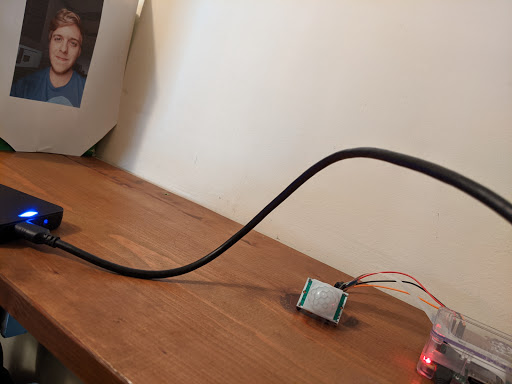
\includegraphics[width=0.7\linewidth]{/Users/hbyadav/Documents/GitHub/IOT/project/ScreenShots/RemoteTesting1.jpg}
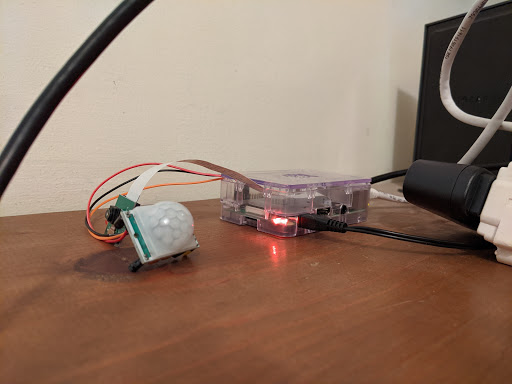
\includegraphics[width=0.7\linewidth]{/Users/hbyadav/Documents/GitHub/IOT/project/ScreenShots/remoteTesting2.jpg}

\section{Face Recognition}
The following sections describe the face recognition algorithms Eigenface, Fisherface, Local binary pattern
histogram and how they are implemented in OpenCV.
\subsection{Eigenface}
Eigenface is based on PCA that classify images to extract features using a set of images. It is important
that the images are in the same lighting condition and the eyes match in each image. Also, images used
in this method must contain the same number of pixels and in grayscale. For this example, consider an
image with n * n pixels as shown in figure 4. Each raw is concatenated to create a vector, resulting a
1*n2 matrix. All the images in the dataset are stored in a single matrix resulting a matrix with columns
corresponding the number of images. The matrix is averaged (normalised) to get an average human face.
By subtracting the average face from each image vector unique features to each face are computed. In
the resulting matrix, each column is a representation of the difference each face has to the average human
face. A simplified illustration can be seen in figure 4.

images goes here

The next step is computing the covariance matrix from the result. To obtain the Eigen vectors from the
data, Eigen analysis is performed using principal component analysis. From the result, where covariance
matrix is diagonal, where it has the highest variance is considered the 1st Eigen vector. 2nd Eigen vector
is the direction of the next highest variance, and it is in 90 degrees to the 1st vector. 3rd will be the
next highest variation, and so on. Each column is considered an image and visualised, resembles a face
and called Eigenfaces. When a face is required to be recognised, the image is imported, resized to match
the same dimensions of the test data as mentioned above. By projecting extracted features on to each
of the Eigenfaces, weights can be calculated. These weights correspond to the similarity of the features
extracted from the different image sets in the dataset to the features extracted from the input image. The
input image can be identified as a face by comparing with the whole dataset. By comparing with each
subset, the image can be identified as to which person it belongs to. By applying a threshold detection
and identification can be controlled to eliminate false detection and recognition. PCA is sensitive to large
numbers and assumes that the subspace is linear. If the same face is analysed under different lighting
conditions, it will mix the values when distribution is calculated and cannot be effectively classified.
This makes to different lighting conditions poses a problem in matching the features as they can change
dramatically.
\subsection{Fisherface}
Fisherface technique builds upon the Eigenface and is based on LDA derived from Ronald Fishers’ linear
discriminant technique used for pattern recognition. However, it uses labels for classes as well as data
point information [6]. When reducing dimensions, PCA looks at the greatest variance, while LDA, using
labels, looks at an interesting dimension such that, when you project to that dimension you maximise
the difference between the mean of the classes normalised by their variance [6]. LDA maximises the ratio
of the between-class scatter and within-class scatter matrices. Due to this, different lighting conditions
in images has a limited effect on the classification process using LDA technique. Eigenface maximises
the variations while Fisherface maximises the mean distance between and different classes and minimises
variation within classes. This enables LDA to differentiate between feature classes better than PCA and
can be observed in figure 5 [12]. Furthermore, it takes less amount of space and is the fastest algorithm
in this project. Because of these PCA is more suitable for representation of a set of data while LDA is
suitable for classification.

image goes here.
\subsection{Local Binary Pattern Histogram}
Local binary patterns were proposed as classifiers in computer vision and in 1990 By Li Wang [4].
The combination of LBP with histogram oriented gradients was introduced in 2009 that increased its
performance in certain datasets [5]. For feature encoding, the image is divided into cells (4 x 4 pixels).
Using a clockwise or counter-clockwise direction surrounding pixel values are compared with the central
as shown in figure 6. The value of intensity or luminosity of each neighbour is compared with the centre
pixel. Depending if the difference is higher or lower than 0, a 1 or a 0 is assigned to the location. The result
provides an 8-bit value to the cell. The advantage of this technique is even if the luminosity of the image

image goes here
is changed as in figure 7, the result is the same as before. Histograms are used in larger cells to find the
frequency of occurrences of values making process faster. By analysing the results in the cell, edges can
be detected as the values change. By computing the values of all cells and concatenating the histograms,
feature vectors can be obtained. Images can be classified by processing with an ID attached. Input
images are classified using the same process and compared with the dataset and distance is obtained. By
setting up a threshold, it can be identified if it is a known or unknown face. Eigenface and Fisherface
compute the dominant features of the whole training set while LBPH analyse them individually.

image goes here:
\section{Methodology}
Below are the methodology and descriptions of the applications used for data gathering, face detection,
training and face recognition. The project was coded in Python using a mixture of IDLE and PYCharm
IDEs.
\subsection{Face Detection}
First stage was creating a face detection system using Haar-cascades. Although, training is required for
creating new Haar-cascades, OpenCV has a robust set of Haar-cascades that was used for the project.
Using face-cascades alone caused random objects to be identified and eye cascades were incorporated to
obtain stable face detection. The flowchart of the detection system can be seen in figure 8. Face and eye

image goes here
classifier objects are created using classifier class in OpenCV through the cv2.CascadeClassifier() and
loading the respective XML files. A camera object is created using the cv2.VideoCapture() to capture
images. By using the CascadeClassifier.detectMultiScale() object of various sizes are matched and
location is returned. Using the location data, the face is cropped for further verification. Eye cascade is
used to verify there are two eyes in the cropped face. If satisfied a marker is placed around the face to
illustrate a face is detected in the location.
\subsection{Face Recognition Process}
For this project three algorithms are implemented independently. These are Eigenface, Fisherface and
Linear binary pattern histograms respectively. All three can be implemented using OpenCV libraries.
There are three stages for the face recognition as follows:
1. Collecting images IDs
2. Extracting unique features, classifying them and storing in XML files
3. Matching features of an input image to the features in the saved XML files and predict identity.
\subsubsection{Collecting the image data}
Collecting classification images is usually done manually using a photo editing software to crop and
resize photos. Furthermore, PCA and LDA requires the same number of pixels in all the images for the
correct operation. This time consuming and a laborious task is automated through an application to
collect 50 images with different expressions. The application detects suitable expressions between 300ms,
straightens any existing tilt and save them. The Flow chart for the application is shown in figure 9.

image goes here

Application starts with a request for a name to be entered to be stored with the ID in a text file. The
face detection system starts the first half. However, before the capturing begins, the application check for
the brightness levels and will capture only if the face is well illuminated. Furthermore, after the face is
detected, the position of the eyes are analysed. If the head is tilted, the application automatically corrects
the orientation. These two additions were made considering the requirements for Eigenface algorithm.
The Image is then cropped and saved using the ID as a filename to be identified later. A loop runs
this program until 50 viable images are collected from the person. This application made data collection
efficient.
\subsubsection{Training the Classifiers}
OpenCV enables the creation of XML files to store features extracted from datasets using the FaceRecognizer class. The stored images are imported, converted to grayscale and saved with IDs in two lists
with same indexes. FaceRecognizer objects are created using face recogniser class. Each recogniser can
take in parameters that are described below:
cv2.face.createEigenFaceRecognizer()
1. Takes in the number of components for the PCA for crating Eigenfaces. OpenCV documentation
mentions 80 can provide satisfactory reconstruction capabilities.
2. Takes in the threshold in recognising faces. If the distance to the likeliest Eigenface is above this
threshold, the function will return a -1, that can be used state the face is unrecognisable
6
cv2.face.createFisherfaceRecognizer()
1. The first argument is the number of components for the LDA for the creation of Fisherfaces.
OpenCV mentions it to be kept 0 if uncertain.
2. Similar to Eigenface threshold. -1 if the threshold is passed.
cv2.face.createLBPHFaceRecognizer()
1. The radius from the centre pixel to build the local binary pattern.
2. The Number of sample points to build the pattern. Having a considerable number will slow down
the computer.
3. The Number of Cells to be created in X axis.
4. The number of cells to be created in Y axis.
5. A threshold value similar to Eigenface and Fisherface. if the threshold is passed the object will
return -1
Recogniser objects are created and images are imported, resized, converted into numpy arrays and stored
in a vector. The ID of the image is gathered from splitting the file name, and stored in another vector.
By using FaceRecognizer.train(NumpyImage, ID) all three of the objects are trained. It must be
noted that resizing the images were required only for Eigenface and Fisherface, not for LBPH. Next, the
configuration model is saved as a XML file using FaceRecognizer.save(FileName). In this project,
all three are trained and saved through one application for convenience. The flow chart for the trainer is
shown in figure 10.

images goes here.

\subsubsection{The Face Recognition}
Face recogniser object is created using the desired parameters. Face detector is used to detect faces in the
image, cropped and transferred to be recognised. This is done using the same technique used for the image
capture application. For each face detected, a prediction is made using FaceRecognizer.predict() which
return the ID of the class and confidence. The process is same for all algorithms and if the confidence
his higher than the set threshold, ID is -1. Finally, names from the text file with IDs are used to display
the name and confidence on the screen. If the ID is -1, the application will print unknown face without
the confidence level. The flow chart for the application is shown in figure 11.

image goes here:

\section{result}
The collected images are shown below. Each face has 50 images. Three applications were written to iter- ate through the parameters of each algorithm. On each iteration, the algorithm is trained using different parameters and tested against a photo. The resulting data is plotted at the after finishing the tests. The applications are :

result goes here.
\section{Conclusions, Limitations and Future Works}
This paper describes the mini-project for visual perception and autonomy module. Next, it explains the technologies used in the project and the methodology used. Finally, it shows the results, discuss the challenges and how they were resolved followed by a discussion. Using Haar-cascades for face detection worked extremely well even when subjects wore spectacles. Real time video speed was satisfactory as well devoid of noticeable frame lag. Considering all factors, LBPH combined with Haar-cascades can be implemented as a cost effective face recognition platform. An example is a system to identify known troublemakers in a mall or a supermarket to provide the owner a warning to keep him alert or for automatic attendance taking in a class.

\end{document}